\subsection{UC2: Autenticazione standard}
\begin{figure}[!ht]
    \caption{Diagramma di UC2: Autenticazione standard}
    \vspace{10px}
    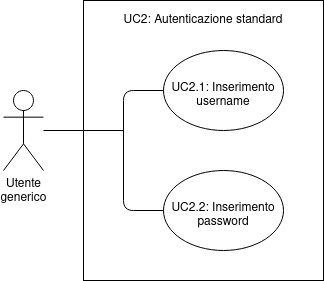
\includegraphics[scale=0.5]{../../../Images/AnalisiRequisiti/UC02}
    \centering
\end{figure}
\label{sec:UC2}
\begin{itemize}
    \item \textbf{Descrizione:} permette l'autenticazione di un utente;
    \item \textbf{Attore Primario:} utente non autenticato;
    \item \textbf{Attore Secondario:} Amazon Cognito;
    \item \textbf{Precondizione:} l'utente è all'interno della pagina di autenticazione;
    \item \textbf{Input:} inserimento dati;
    \item \textbf{Postcondizione:} l'utente è autenticato;
    \item \textbf{Scenario Principale:}
          \begin{itemize}
              \item l'utente è nella pagina dedicata all'autenticazione;
              \item inserisce i propri dati;
              \item preme l'apposito bottone;
              \item l'utente è autenticato.
          \end{itemize}
          \textbf{Estensione:}
          Se lo username o la password non sono corretti:
          \begin{itemize}
              \item viene visualizzato un messaggio di errore (\hyperref[sec:UC33]{\underline{UC33}});
              \item si può ritentare l'inserimento dei dati.
          \end{itemize}
\end{itemize}
\subsubsection{UC2.1: Inserimento username}
\label{sec:UC2.1}
\begin{itemize}
    \item \textbf{Descrizione:} permette l'inserimento dell'username;
    \item \textbf{Attore Primario:} utente non autenticato;
    \item \textbf{Attore Secondario:} Amazon Cognito;
    \item \textbf{Precondizione:} l'utente è all'interno della pagina di autenticazione
    \item \textbf{Input:} inserimento username;
    \item \textbf{Postcondizione:} l' username è stato inserito.
\end{itemize}
\subsubsection{UC2.2: Inserimento password}
\label{sec:UC2.2}
\begin{itemize}
    \item \textbf{Descrizione:} permette l'inserimento della password;
    \item \textbf{Attore Primario:} utente non autenticato;
    \item \textbf{Attore Secondario:} Amazon Cognito;
    \item \textbf{Precondizione:} l'utente è all'interno della pagina di autenticazione;
    \item \textbf{Input:} inserimento password;
    \item \textbf{Postcondizione:} la password è stata inserita.
\end{itemize}

